\documentclass[usenames,dvipsnames,svgnames,table]{beamer}

\usetheme{AnnArbor} %was there really a choice?
\usepackage{lmodern}
\usepackage{amsmath}
\usepackage{enumitem}
\usepackage{multicol}
\usepackage{graphicx}
\usepackage{epstopdf}
\usepackage{pgffor}
\usepackage{rotating}

\newcommand{\experiment}[1]{\textcolor{blue}{#1}}
\newcommand{\CMS}[1]{\experiment{#1}}
\newcommand{\ATLAS}[1]{\experiment{#1}}
\newcommand{\theory}[1]{\textcolor{red}{#1}}
\newcommand{\dontknow}[1]{\textcolor{cyan}{#1}}
\newcommand{\me}[1]{\textbf{\CMS{#1}}}
\newcommand{\arxiv}[1]{\href{http://arxiv.org/abs/#1}{\nolinkurl{arXiv:#1}}}
\newcommand{\snowmass}{\arxiv{1309.4819}}

\newcommand{\spin}[1]{\text{spin }#1}
\renewcommand{\therefore}{\Rightarrow}

\newenvironment{variableblock}[3]{
%http://tex.stackexchange.com/questions/33231/how-to-change-the-color-of-a-block-within-a-custom-beamer-sty-theme-file
  \setbeamercolor{block body}{#2}
  \setbeamercolor{block title}{#3}
  \begin{block}{#1}\end{block}}

\title[JHUGen and MELA]{Tools for the Higgs boson CP studies: \\ JHUGen and MELA}

\author[Heshy Roskes]{\CMS{I.~Anderson}, \CMS{S.~Bolognesi}, \theory{F.~Caola}, \ATLAS{Y.~Gao}, \CMS{A.~Gritsan}, \CMS{Z.~Guo}, \CMS{C.~Martin}, \theory{K.~Melnikov}, \me{Heshy~Roskes}, \CMS{U.~Sarica}, \theory{M.~Schulze}, \CMS{N.~Tran}, \CMS{A.~Whitbeck}, \CMS{M.~Xiao}, \CMS{C.~You}, \theory{Y.~Zhou}
\texorpdfstring{
\\Johns Hopkins University\\ \leavevmode \\
\theory{Theory}, \experiment{experiment}}{}}

\date[August 4, 2015]{2015 meeting, APS Division of Particles and Fields\\
Ann Arbor, MI \\ \leavevmode \\
August 4, 2015}

%\author{I.~Anderson, S.~Bolognesi, F.~Caola, Y.~Gao, A.~Gritsan, C.~Martin, Z.~Guo, K.~Melnikov, {H.~Roskes}, U.~Sarica, M.~Schulze, N.~Tran, A.~Whitbeck, M.~Xiao, C.~You, Y.~Zhou}



\begin{document}

\begin{frame}
\titlepage
\end{frame}

\begin{frame}{Framework}

\begin{itemize}
\small
\item JHUGen
\begin{itemize}
\item Event generation
\end{itemize}
\item JHUGenMELA
\begin{itemize}
\item Discriminants for anomalous coupling fits and background suppression
\item Reweighting
\end{itemize}
\item AnalyticMELA
\begin{itemize}
\item Discriminants for anomalous coupling fits and background suppression
\item Analytic multidimensional fits
\item Validation
\end{itemize}
\item
\item \url{http://www.pha.jhu.edu/spin/}
\begin{itemize}
\item \arxiv{1001.3396}
\item \arxiv{1208.4018}
\item \snowmass
\end{itemize}
\end{itemize}

\end{frame}


\begin{frame}{JHU Generator}
\begin{itemize}
\begin{multicols}{2}
\item $gg\to H$
\item $gg/gq\to H+\text{jet}$
\item $gg/gq/qq^\prime\to H+2\text{ jets}$ (QCD)
\item $qq^\prime\to H+2\text{ jets}$ (VBF)
\item $q\bar{q}\to Z^*\to Z+H$
\item $q\bar{q}^\prime\to W^*\to W+H$
\item $gg/q\bar{q}\to t\bar{t}H$
\begin{itemize}
\item $t\to Wb \to l\nu b/q\bar{q}^\prime b$
\end{itemize}
\item $q\bar{q}\to\spin{1}$
\item $gg/q\bar{q}\to\spin{2}$
\item Interface to MCFM for $gg\to ZZ$ offshell with anomalous couplings
\end{multicols}
\item Decay:
\begin{itemize}[label={$\to$}] \small
\item \(ZZ^*+Z\gamma^*+\gamma^*\gamma^*\to \text{any combination of $l^+l^-$, $\nu\bar{\nu}$, $q\bar{q}$}\)
\item \(W^+W^-\to \text{any combination of $l\nu$ and $q\bar{q}^\prime$}\)
\item $Z\gamma$, $\gamma\gamma$
\end{itemize}
\item Production and decay in one step for spin 1 and spin 2
\item \texttt{ReadLHE} mode for other processes or to decay events from other generators
\end{itemize}
\end{frame}

\begin{frame}{Parameterization}
\begin{itemize}
%\item Most general parameterization of anomalous couplings:
\item \small
$
A(HVV) \sim
$
\begin{itemize}
\item
$
\left[ a_{1}
+ \textcolor{Green}{\frac{q_{V_1}^2 +  q_{V_2}^{2}}{\left(\Lambda_{1} \right)^{2}}}
+ \textcolor{magenta}{\frac{(q_{V_1} + q_{V_2})^{2}}{\left(\Lambda_{Q} \right)^{2}}}
\right]
m_{V_1}^2 \epsilon_{V_1}^* \epsilon_{V_2}^*
+ \textcolor{red}{a_{2}  f_{\mu \nu}^{*(1)}f^{*(2),\mu\nu}}
+ \textcolor{blue}{a_{3}   f^{*(1)}_{\mu \nu} {\tilde f}^{*(2)\mu\nu}}
$
\end{itemize}
%\normalsize Lagrangian (equivalent)
\tiny
\item
$
 {L}(HVV) \sim
$
\begin{itemize}
\item
$
a^{ZZ}_{1}\frac{m_{Z}^2}{2} H Z^{\mu}Z_{\mu}
- \textcolor{Green}{\frac{1}{\left(\Lambda^{ZZ}_{1}\right)^{2}} m_{Z}^2 H  Z^{\mu} \Box Z_{\mu}}
- \textcolor{magenta}{\frac{1}{2\left(\Lambda^{ZZ}_{Q}\right)^{2}} m_{Z}^2 \Box H  Z^{\mu} Z_{\mu}}
- \textcolor{red}{\frac{1}{2}a^{ZZ}_{2} H  Z^{\mu\nu}Z_{\mu\nu}}
- \textcolor{blue}{\frac{1}{2}a^{ZZ}_{3} H  Z^{\mu\nu}{\tilde Z}_{\mu\nu}}
$
\item
$
+ a_{1}^{WW}{m_{W}^2} H W^{+\mu} W^{-}_{\mu}
- \textcolor{Green}{\frac{1}{\left(\Lambda_{1}^{WW}\right)^{2}} m_{W}^2 H
  \left(  W^{-}_{\mu} \Box W^{+\mu} + W^{+}_{\mu} \Box W^{-\mu} \right)}
$
\begin{itemize}
\item
$
- \textcolor{magenta}{\frac{1}{\left(\Lambda_{Q}\right)^{2}} m_{W}^2 \Box H  W^{+\mu} W^{-}_{\mu}}
- \textcolor{red}{a_{2}^{WW} H W^{+\mu\nu}W^{-}_{\mu\nu}}
- \textcolor{blue}{a_{3}^{WW} H W^{+\mu\nu}{\tilde W}^{-}_{\mu\nu}}
$
\end{itemize}
\item
$
+ \textcolor{Green}{\frac{1}{\left(\Lambda_{1}^{Z\gamma} \right)^{2}} m_{Z}^2 H  Z_\mu \partial_\nu F^{\mu\nu}}
- \textcolor{red}{a_{2}^{Z\gamma} H F^{\mu\nu} Z_{\mu\nu}}
- \textcolor{blue}{a_{3}^{Z\gamma} H  F^{\mu\nu}{\tilde Z}_{\mu\nu}}
$
\item
$
- \textcolor{red}{\frac{1}{2}a_{2}^{\gamma\gamma} H  F^{\mu\nu}F_{\mu\nu}}
- \textcolor{blue}{\frac{1}{2}a_{3}^{\gamma\gamma}H  F^{\mu\nu}{\tilde F}_{\mu\nu}}
$
\item
$
- \textcolor{red}{\frac{1}{2}a_{2}^{gg} H  G^{\mu\nu}_a G^a_{\mu\nu}}
- \textcolor{blue}{\frac{1}{2}a_{3}^{gg}H  G^{\mu\nu}_a{\tilde G}^a_{\mu\nu}}
$
\end{itemize}
\item \small Similar for spin 1 and spin 2, and similar terms for fermion couplings
\item
\item Predictions are leading order QCD
\item POWHEG (NLO QCD) $gg\to H$ $\longrightarrow$ JHUGen anomalous decay
\begin{itemize}
\item Anomalous couplings do not affect 1 jet correlations
\end{itemize}
\end{itemize}
\end{frame}

\begin{frame}{JHUGenMELA}{\textcolor{red}{M}atrix \textcolor{red}{E}lement \textcolor{red}{L}ikelihood \textcolor{red}{A}pproach}

\begin{itemize}
\item Library including matrix elements for all presented processes
\begin{multicols}{3}
\begin{itemize}
\tiny
\item \texttt{EvalAmp\_gg\_H\_VV} \item \texttt{EvalAmp\_H\_VV} \item \texttt{EvalAmp\_VHiggs} \item \texttt{EvalAmp\_qqb\_Zprime\_VV \item
EvalAmp\_Zprime\_VV} \item \texttt{EvalAmp\_gg\_G\_VV} \item \texttt{EvalAmp\_qqb\_G\_VV} \item \texttt{EvalAmp\_G\_VV \item
EvalAmp\_WBFH} \item \texttt{EvalAmp\_SBFH} \item \texttt{EvalAmp\_HJ} \item \texttt{EvalXSec\_PP\_TTBH \item
EvalAmp\_GG\_TTBH} \item \texttt{EvalAmp\_QQB\_TTBH}
\item %blank for alignment
\end{itemize}
\end{multicols}
\item Complemented and validated by AnalyticMELA
\item Interface to MCFM for offshell production with anomalous couplings and $ZZ/Z\gamma/\gamma\gamma$ SM background \tiny [Campbell, Ellis, Williams] \normalsize
\item Can be used for:
\begin{itemize}[label=-]
\item optimal discriminants for anomalous coupling fits
\item background suppression
\item reweighting
\end{itemize}
\end{itemize}
\end{frame}

\begin{frame}{Reweighting with JHUGenMELA}
\begin{tabular}{ll}
Basic idea: & $\text{weight}\left(d\Pi\right)=\frac{P(J^P_\text{target},d\Pi)}{P(J^P_\text{sample},d\Pi)}$ \\
& $d\Pi = \begin{cases} \theta^*, \theta_1, \theta_2, \phi, \phi_1, m_1, m_2, m_H \\ p_1, p_2, p_3, p_4 \end{cases}$ \\
For reweighting, & $d\Pi = d\Pi_\text{generator}$ \\
(For fitting, & $d\Pi = d\Pi_\text{observed}$) \\
& \\
Probability distribution: & $P\sim\left|\mathcal{M}\left(d\Pi\right)\right|^2$ \\
 & or $\sim f^p_i\left(x_1\right)f^p_j(x_2)\left|\mathcal{M}\left(d\Pi\right)\right|^2$

\end{tabular}
\end{frame}

\begin{frame}{Validation of reweighting}{Compare reweighted sample vs. dedicated production}
\centering
\includegraphics[width=0.4\textwidth]{reweightingvalidation/fa2halffa31} %\hfill
\includegraphics[width=0.4\textwidth]{reweightingvalidation/fa2halffa3half}\\
\includegraphics[width=0.4\textwidth]{reweightingvalidation/fa2Zgamma} %\hfill
\includegraphics[width=0.4\textwidth]{reweightingvalidation/flambda1fa3Zgamma}
\end{frame}

\begin{frame}{$HVV$ vertex kinematics}{\snowmass}

\begin{columns} \small
\begin{column}{0.33\textwidth} \centering
\includegraphics[width=\columnwidth]{snowmass/angles-HZZ4l} \\
\[\phantom{equation=ghost}\]
\[\left[gg\to\right] H\to ZZ\to 4l\]
\end{column}
\begin{column}{0.33\textwidth} \centering
\includegraphics[width=\columnwidth]{snowmass/angles-ZZHBB} \\
\[q\bar{q}\to Z^*\to ZH\]
\[Z\to l^+l^- \left[H\to b\bar{b}\right]\]
\end{column}
\begin{column}{0.33\textwidth} \centering
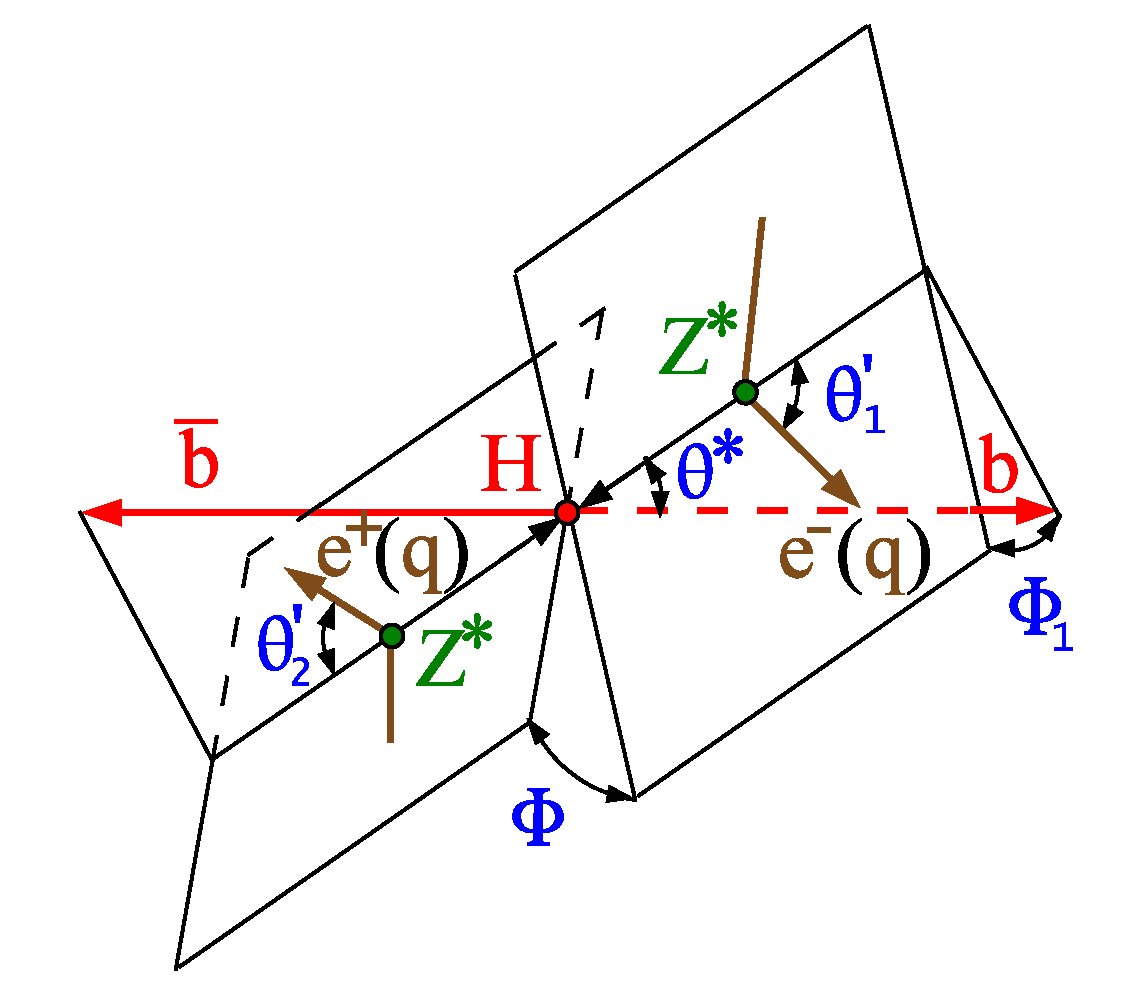
\includegraphics[width=\columnwidth]{snowmass/angles-HZZVBF} \\
\[\text{VBF}\]
\[qq^\prime\to Z^*Z^*\to H\left[\to b\bar{b}\right]\]
\end{column}
\end{columns}
\vfill
\end{frame}

\begin{frame}{Applications for discriminating spin and CP properties}{$H\to ZZ\to 4l$ decay\hfill \arxiv{1208.4018}}
\begin{tabular}{m{0.10\textwidth}m{0.18\textwidth}m{0.18\textwidth}m{0.18\textwidth}m{0.18\textwidth}}
\footnotesize\centering Spin 0 \tiny \textcolor{red}{$0^+$} \textcolor{blue}{$0^-$} \textcolor{Green}{$0_h^+$} &
\noindent\includegraphics[width=0.18\textwidth]{onthespinandparity/phi_125GeV_spin0} &
\noindent\includegraphics[width=0.18\textwidth]{onthespinandparity/costhetastar_125GeV_spin0} &
\noindent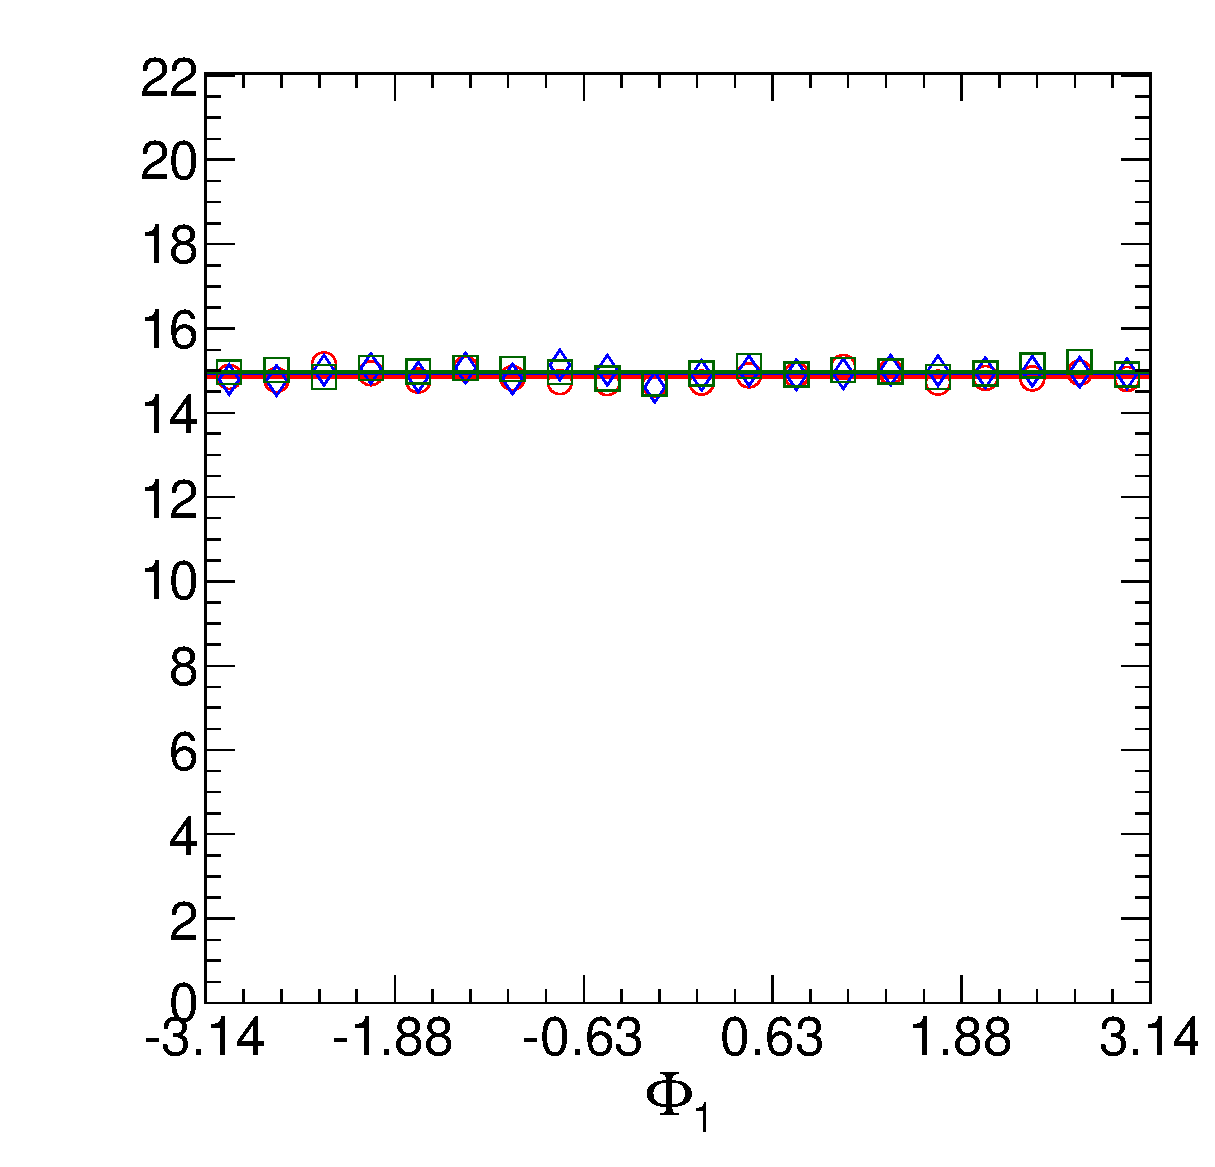
\includegraphics[width=0.18\textwidth]{onthespinandparity/phistar1_125GeV_spin0} &
\noindent\includegraphics[width=0.18\textwidth]{onthespinandparity/costheta1_125GeV_spin0} \\
\footnotesize\centering Spin 1 \tiny \textcolor{red}{$1^+$} \textcolor{blue}{$1^-$} \textcolor{Green}{$1_h^+$} &
\noindent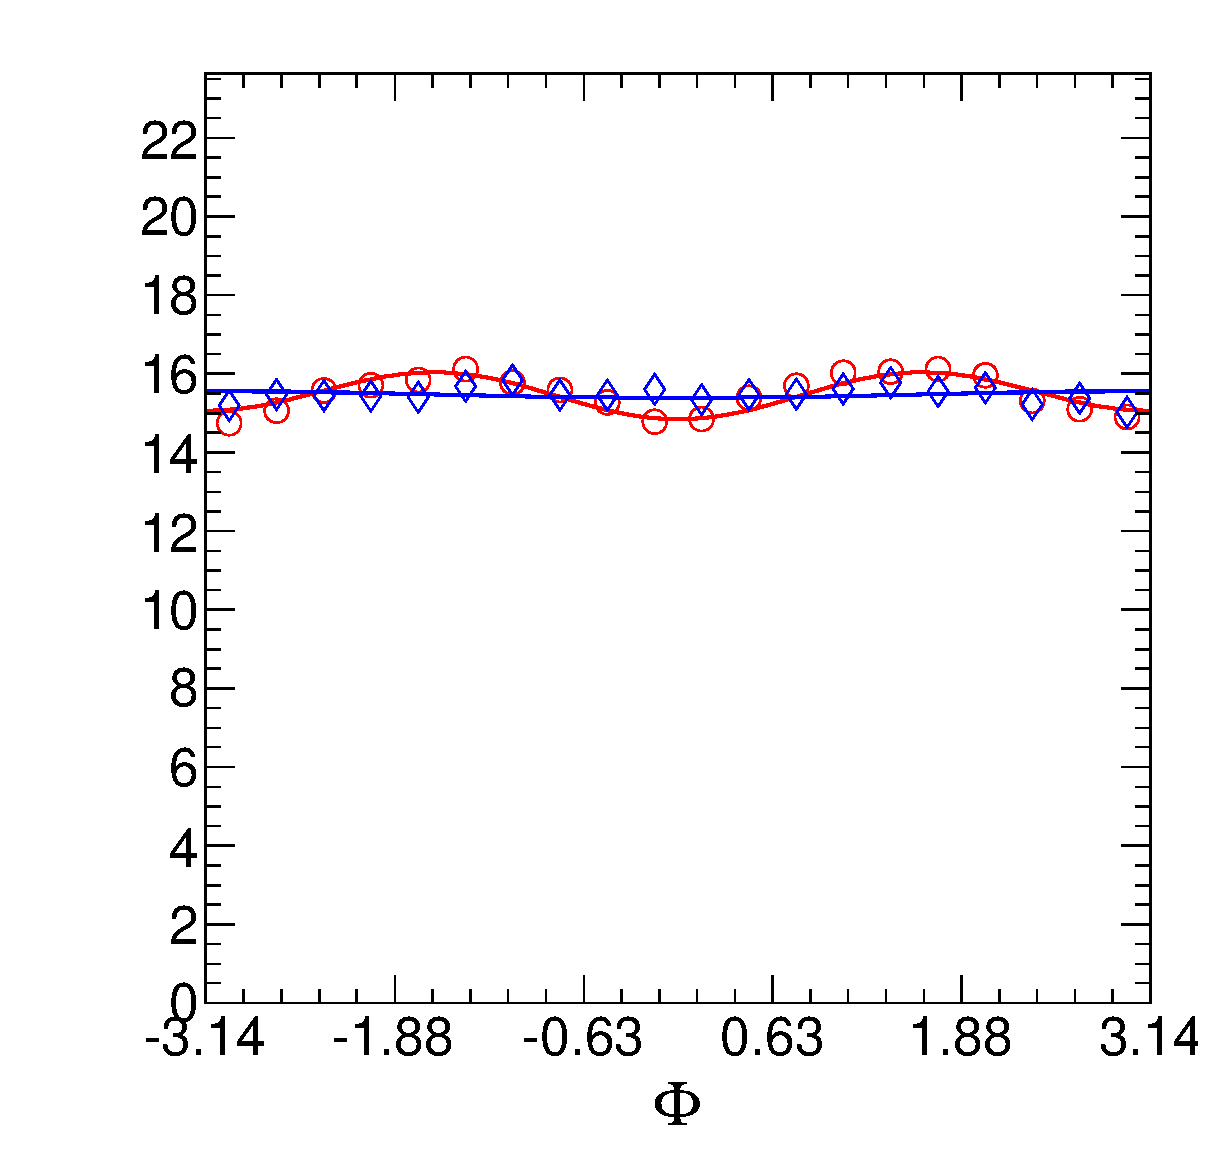
\includegraphics[width=0.18\textwidth]{onthespinandparity/phi_125GeV_spin1} &
\noindent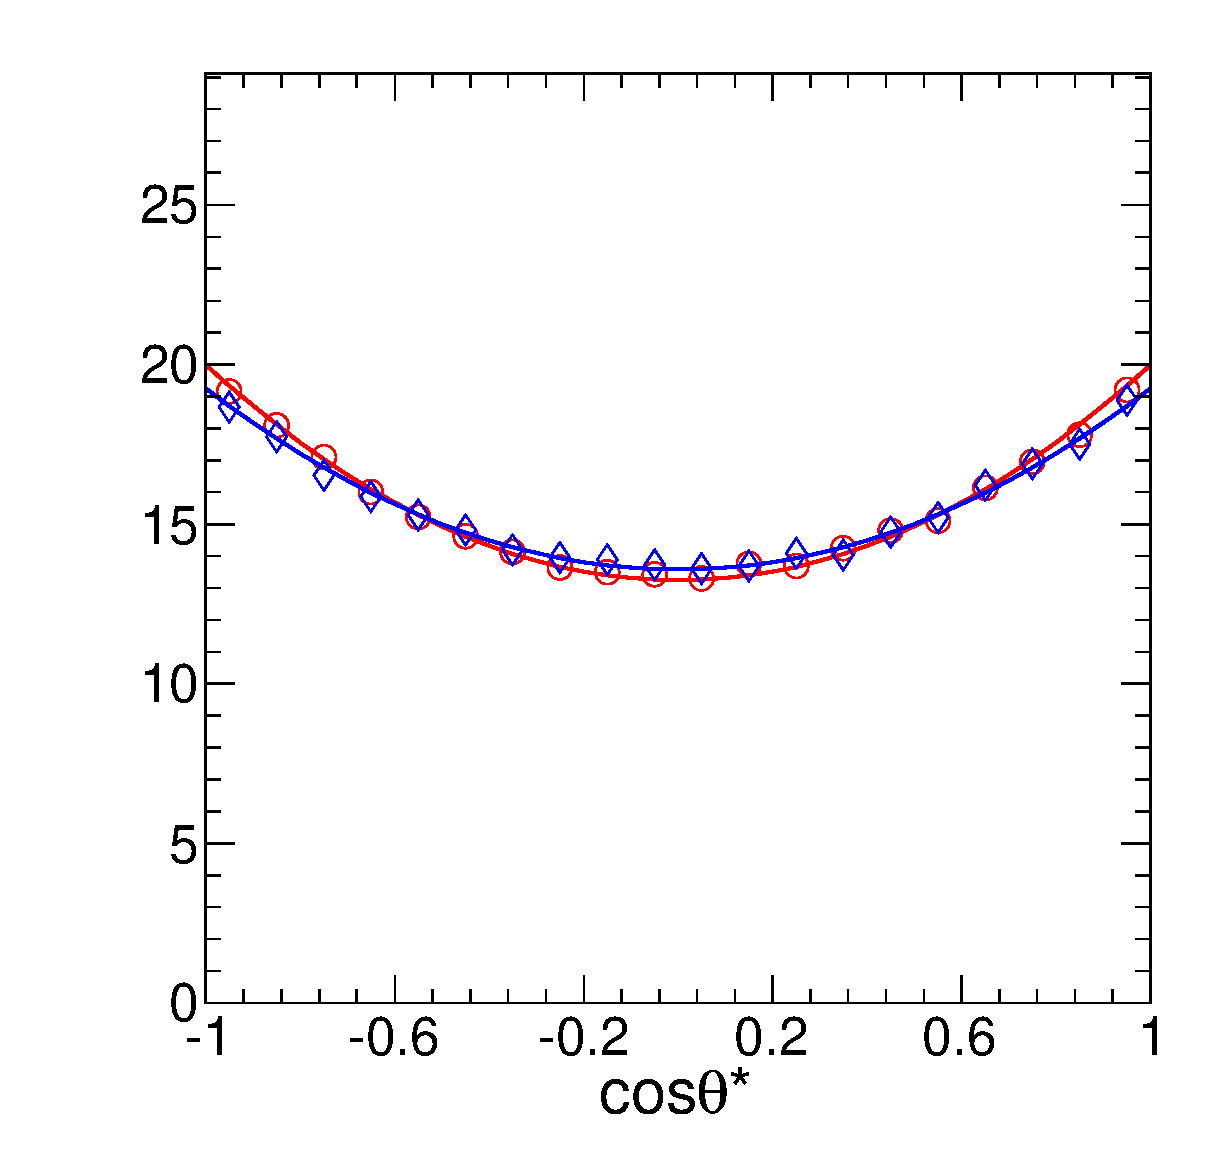
\includegraphics[width=0.18\textwidth]{onthespinandparity/costhetastar_125GeV_spin1} &
\noindent\includegraphics[width=0.18\textwidth]{onthespinandparity/phistar1_125GeV_spin1} &
\noindent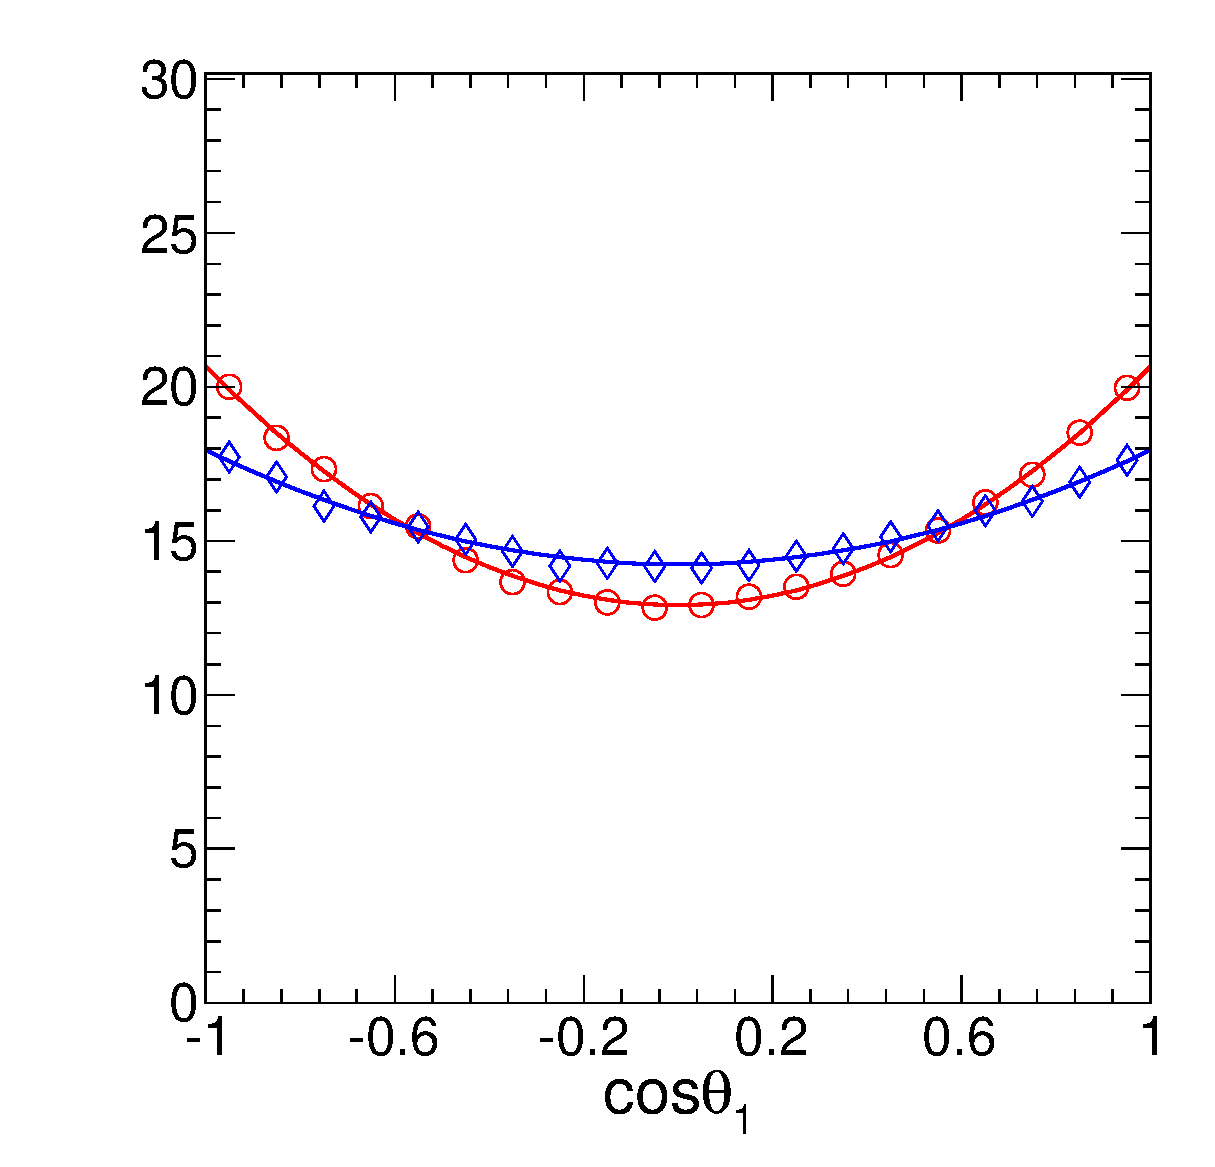
\includegraphics[width=0.18\textwidth]{onthespinandparity/costheta1_125GeV_spin1} \\
\footnotesize\centering Spin 2 \tiny \textcolor{red}{$2^+$} \textcolor{blue}{$2^-$} \textcolor{Green}{$2_h^+$} &
\noindent\includegraphics[width=0.18\textwidth]{onthespinandparity/phi_125GeV_spin2} &
\noindent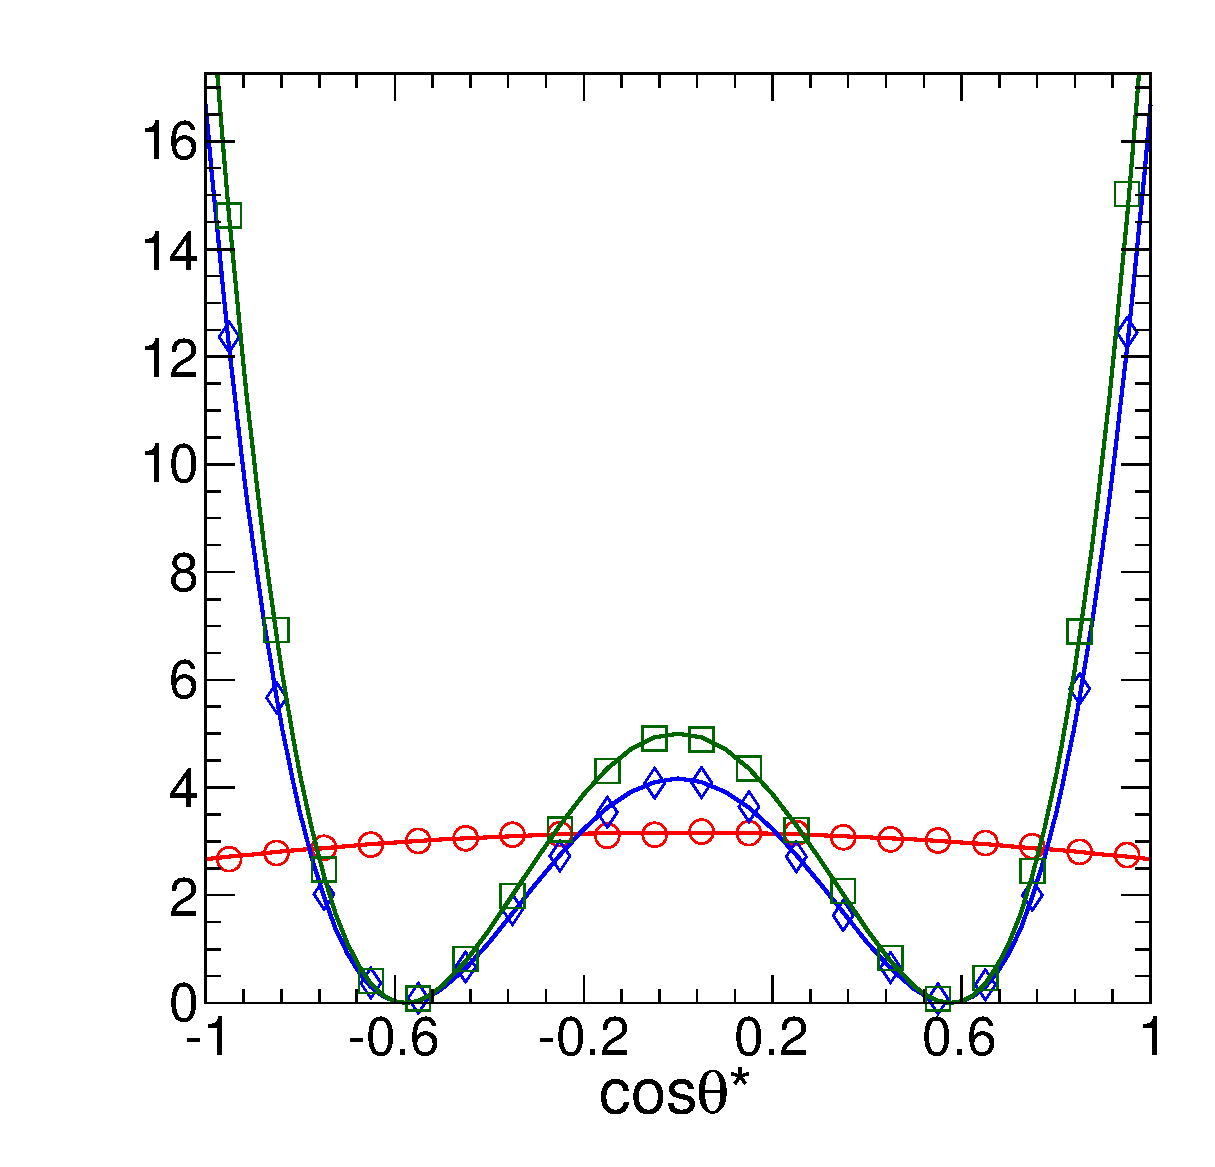
\includegraphics[width=0.18\textwidth]{onthespinandparity/costhetastar_125GeV_spin2}&
\noindent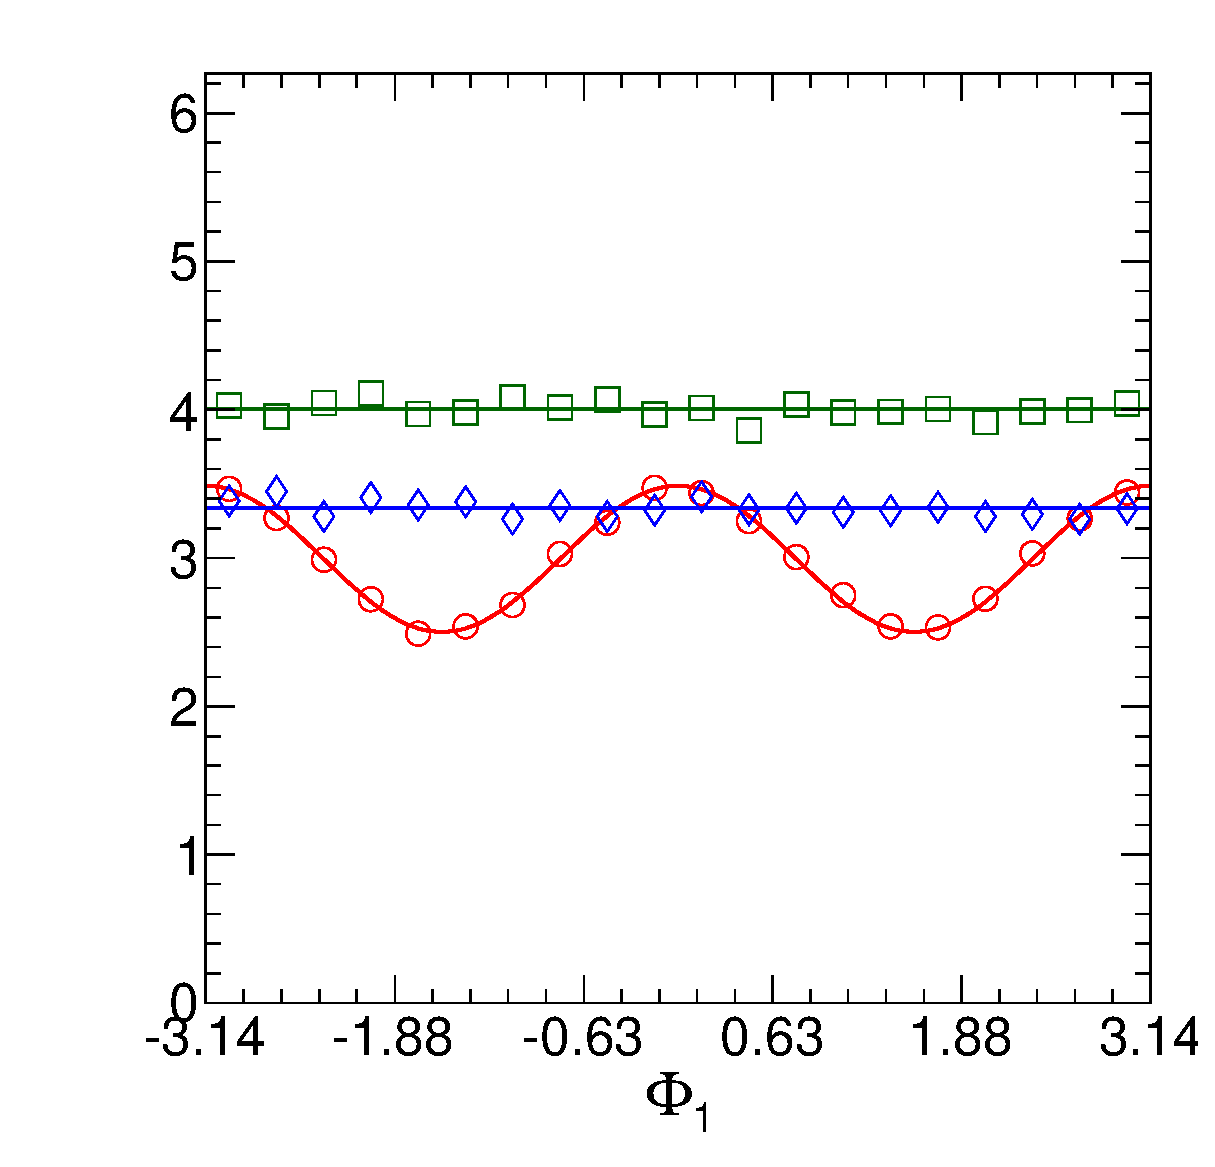
\includegraphics[width=0.18\textwidth]{onthespinandparity/phistar1_125GeV_spin2} &
\noindent\includegraphics[width=0.18\textwidth]{onthespinandparity/costheta1_125GeV_spin2}
\end{tabular}
\end{frame}

\begin{frame}{Applications for discriminating CP properties}{$VH$\hfill\snowmass}
\textcolor{red}{SM} \hfill \textcolor{blue}{$f_{a3}=1$ (pseudoscalar)} \hfill \textcolor{Green}{$f_{a3}=0.5, \phi_{a3}=0$} \hfill \textcolor{magenta}{$f_{a3}=0.5, \phi_{a3}=\pi/2$}
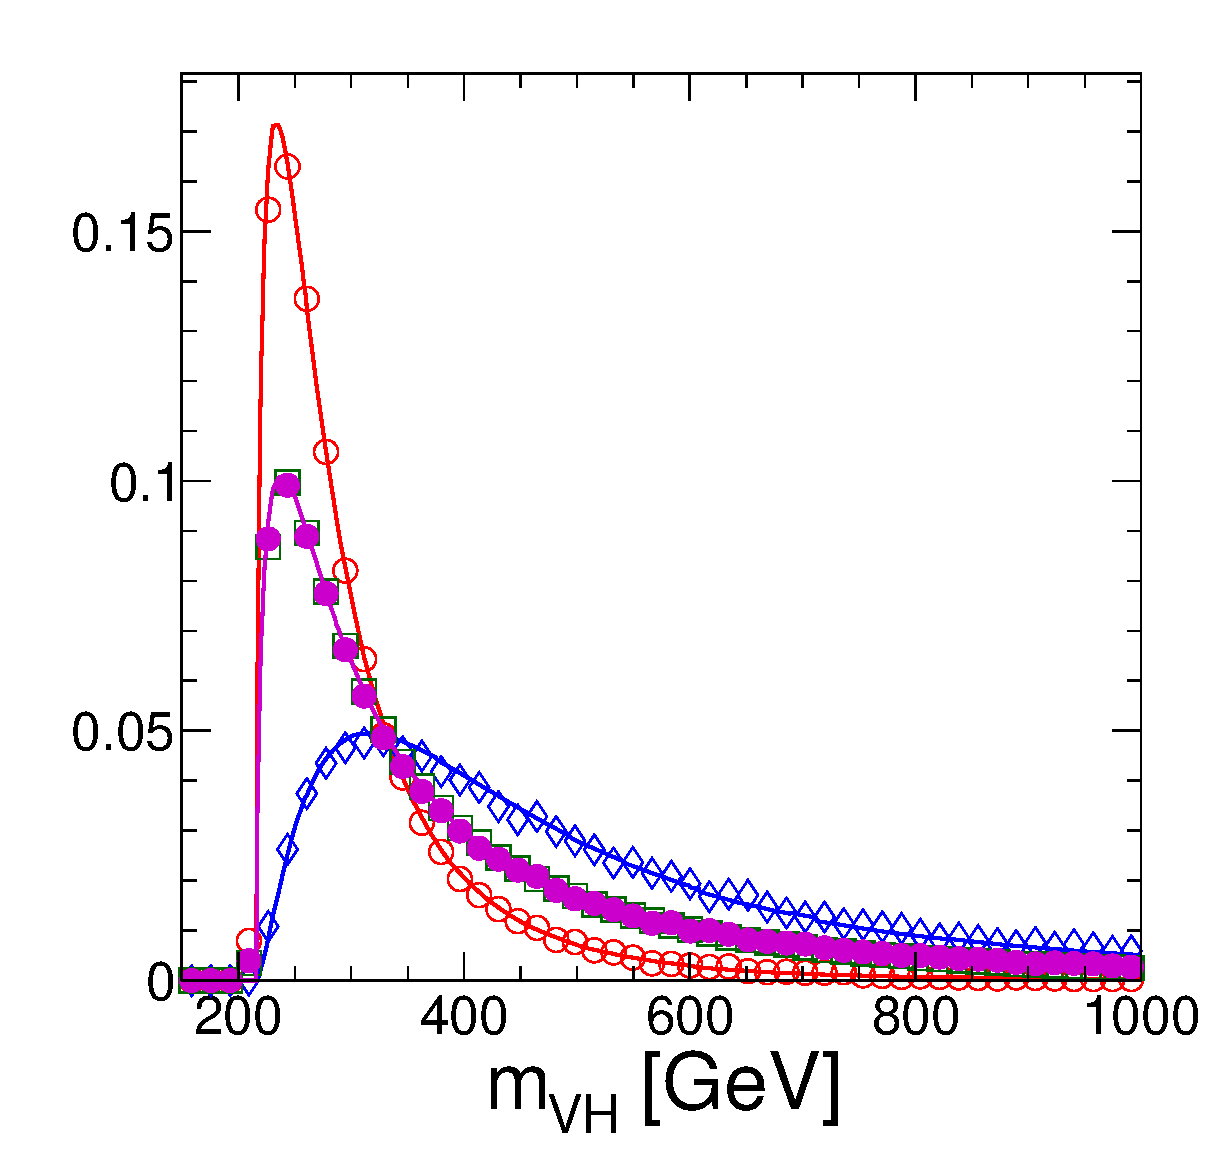
\includegraphics[width=.25\textwidth]{snowmass/ZH_mvh}
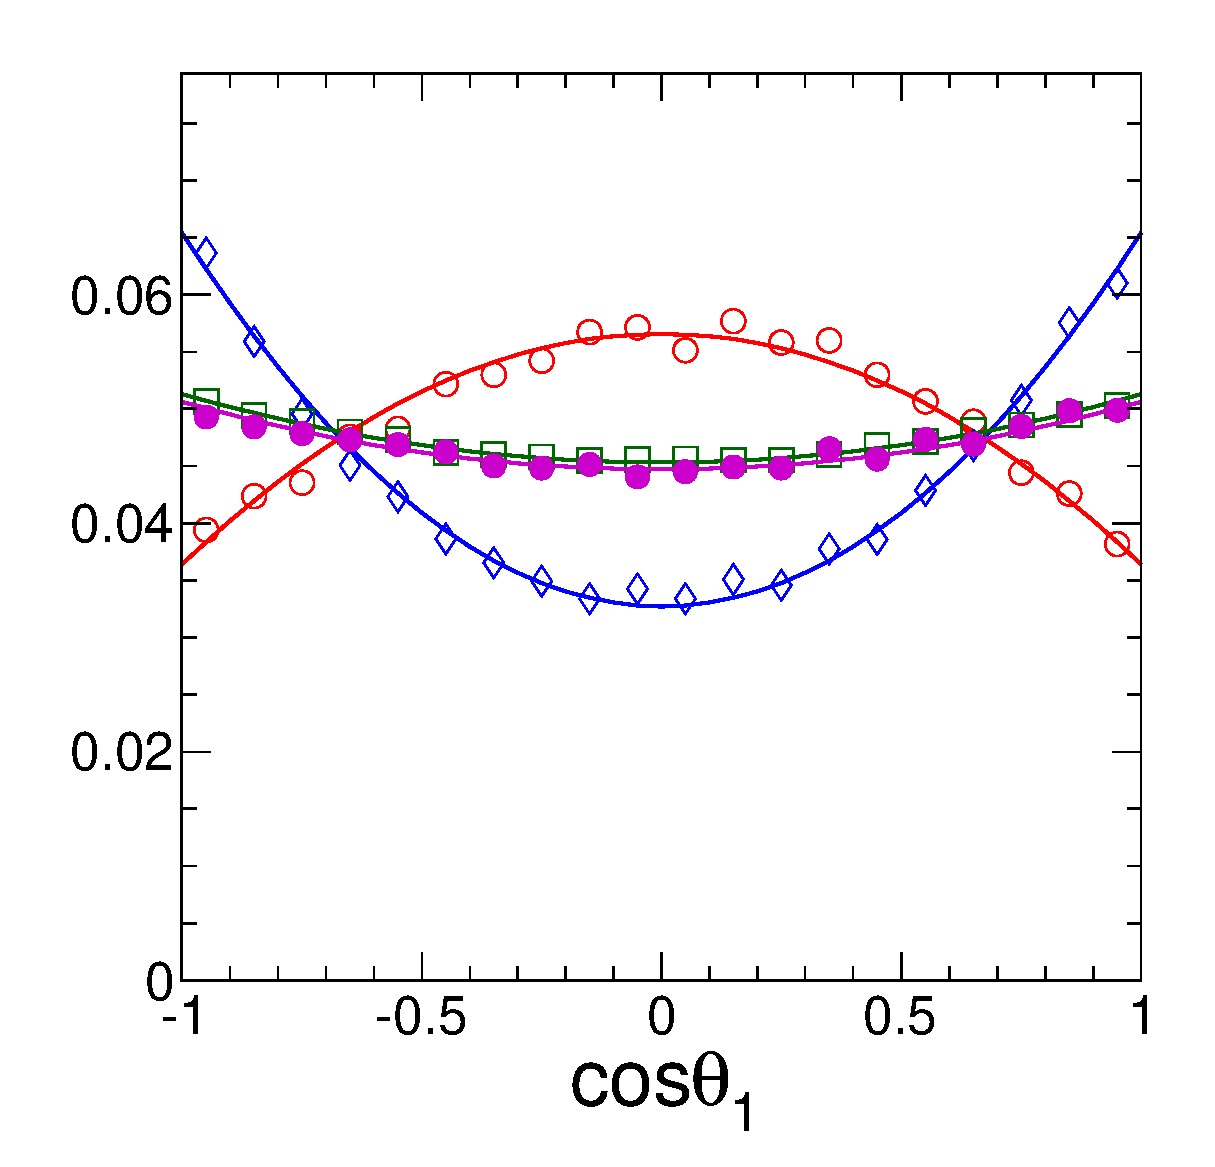
\includegraphics[width=.25\textwidth]{snowmass/ZH_h1}
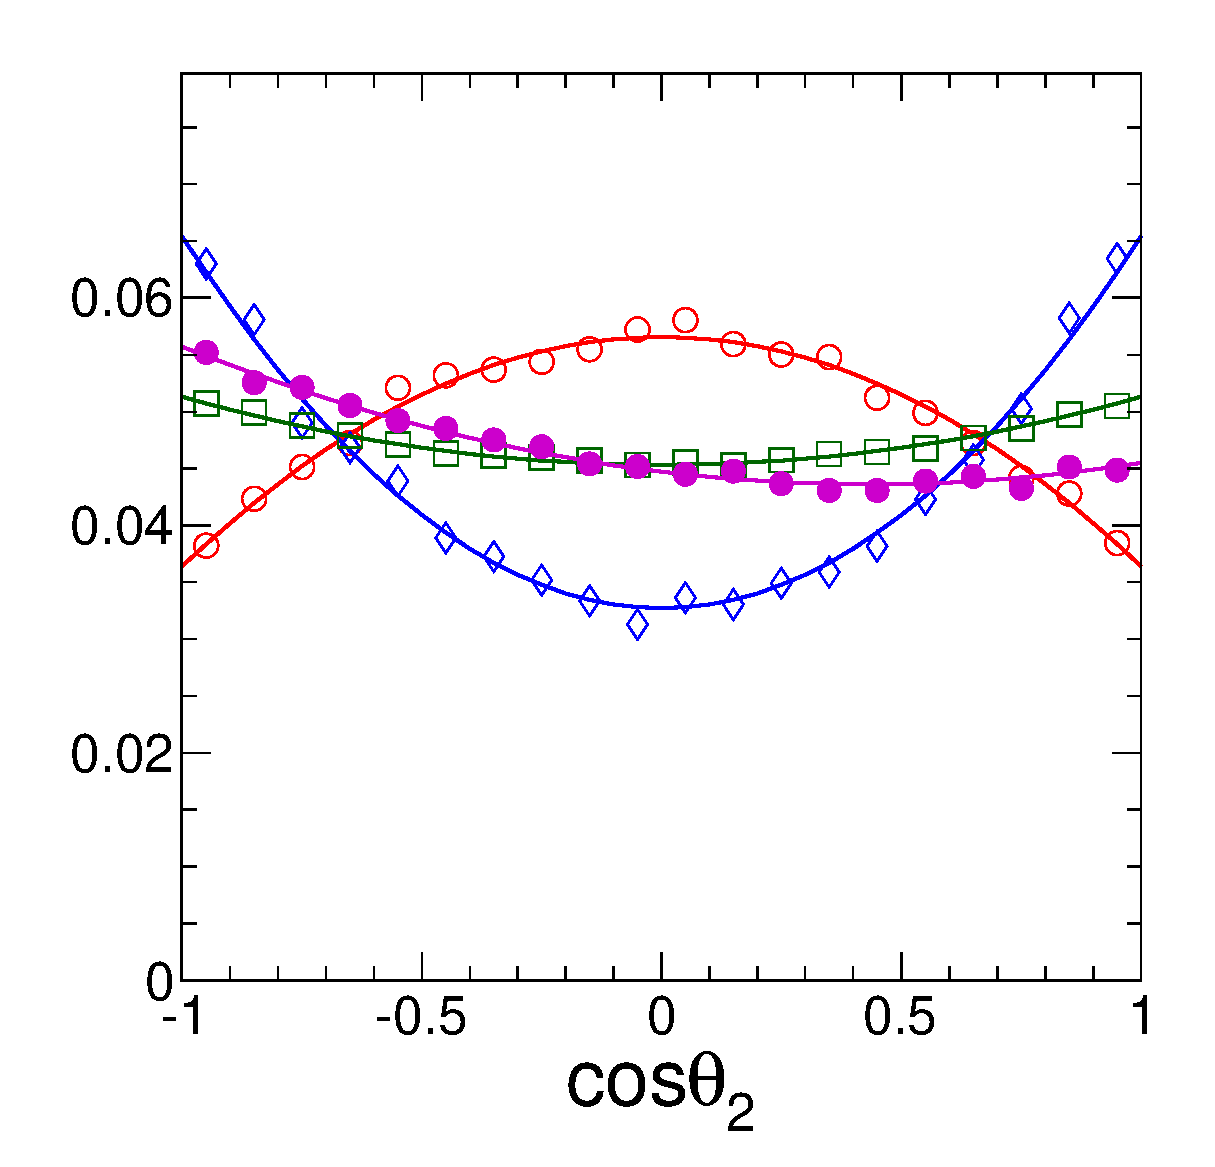
\includegraphics[width=.25\textwidth]{snowmass/ZH_h2}
\includegraphics[width=.25\textwidth]{snowmass/ZH_Phi}
\end{frame}

\begin{frame}{Applications for discriminating CP properties}{VBF\hfill\snowmass}
\textcolor{red}{SM} \hfill \textcolor{blue}{$f_{a3}=1$ (pseudoscalar)} \hfill \textcolor{Green}{$f_{a3}=0.5, \phi_{a3}=0$} \hfill \textcolor{magenta}{$f_{a3}=0.5, \phi_{a3}=\pi/2$}
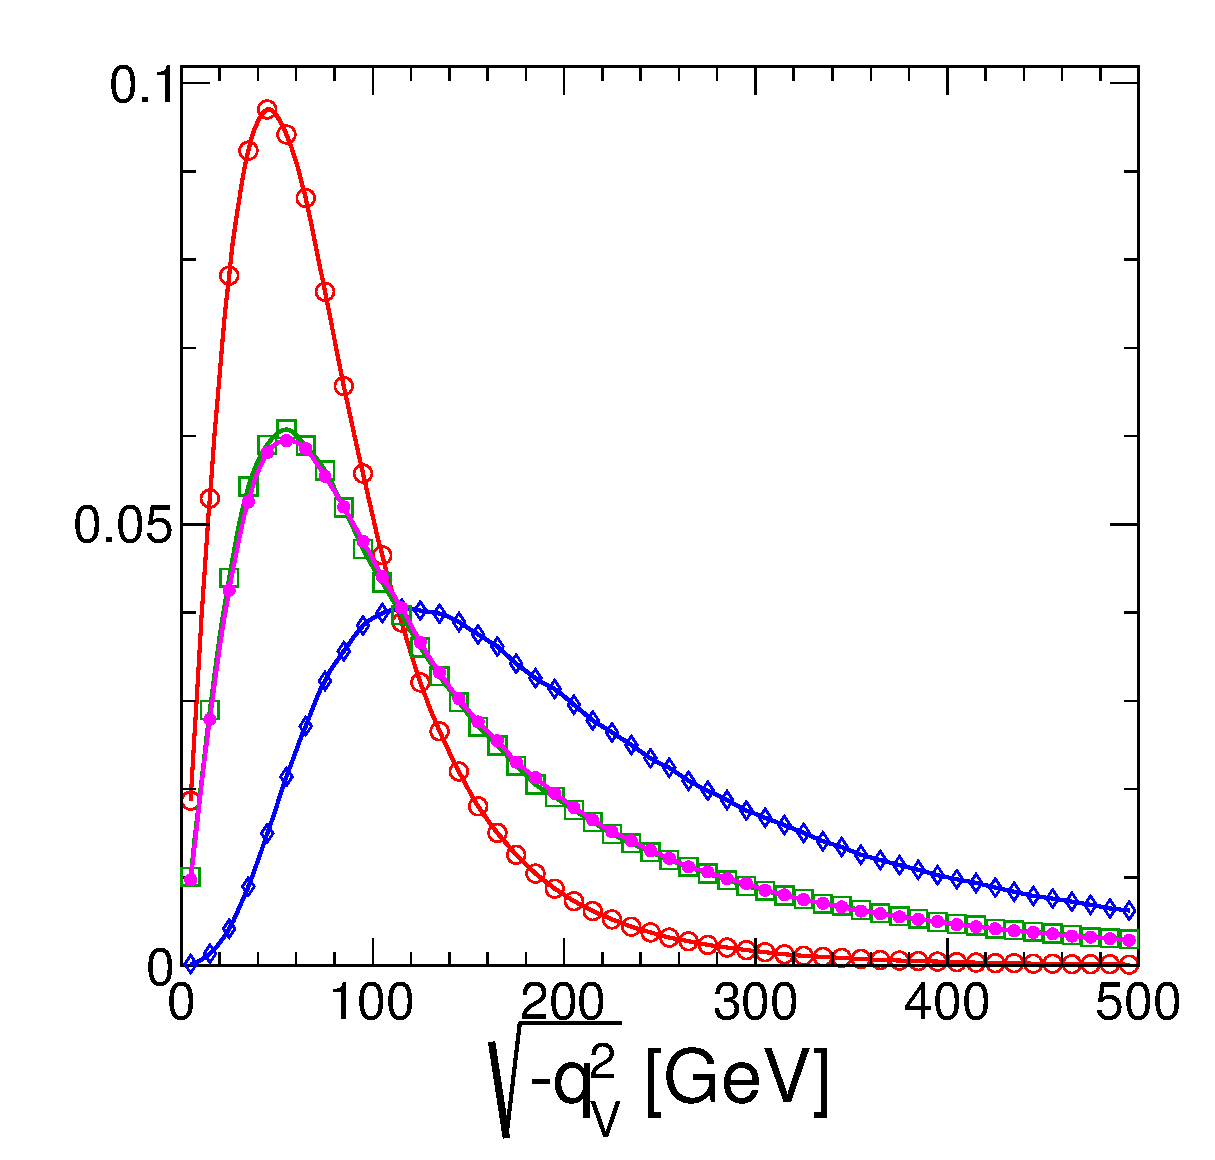
\includegraphics[width=.25\textwidth]{snowmass/14T_WBF_Q2_50}
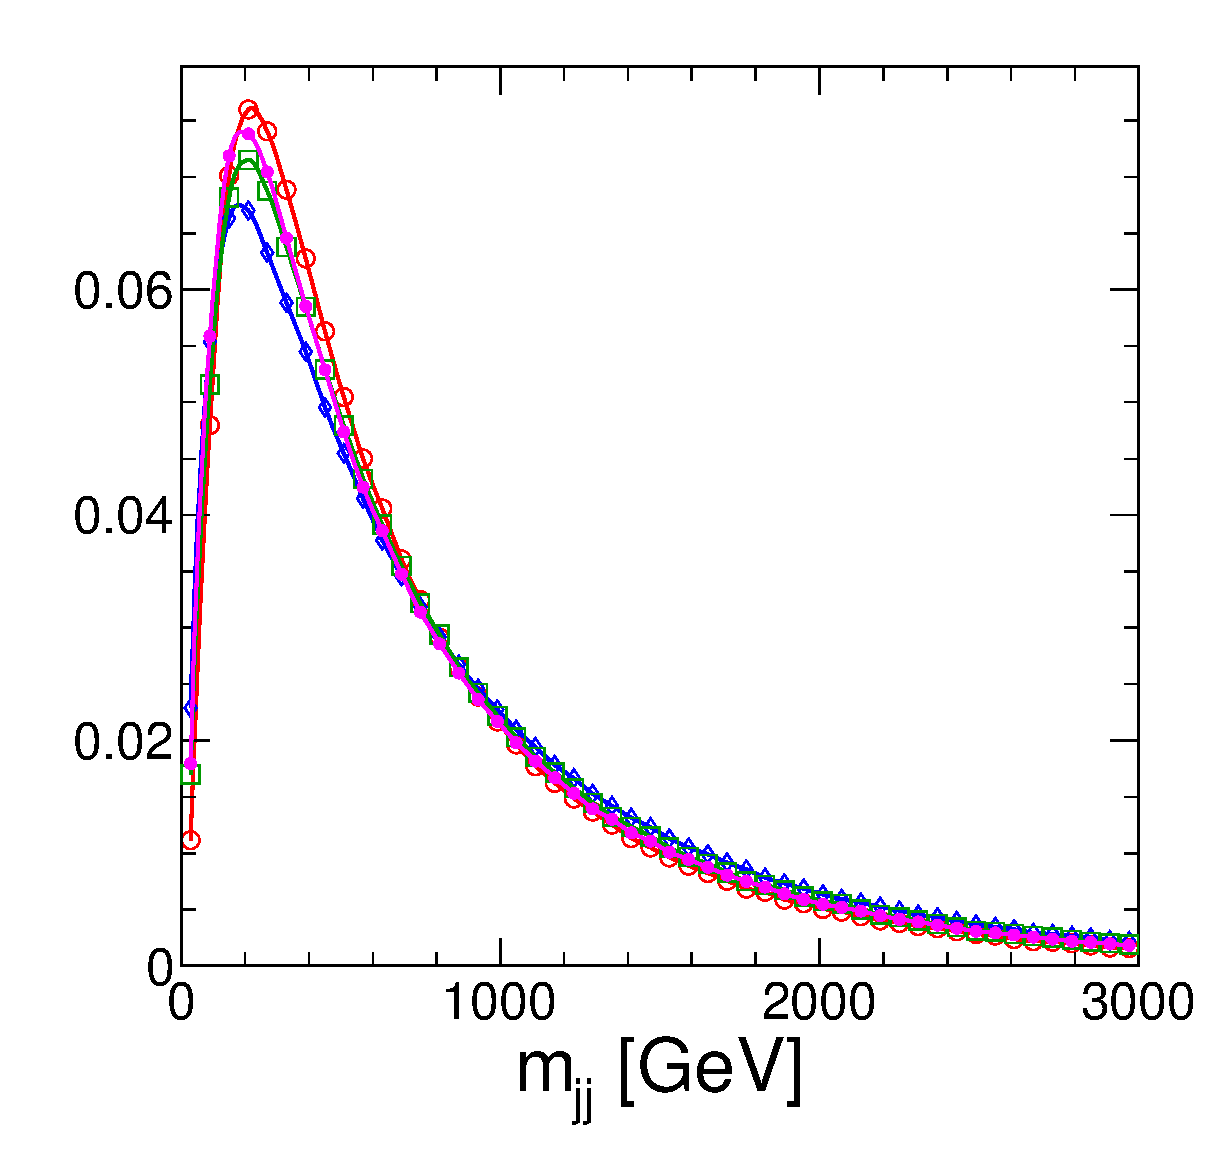
\includegraphics[width=.25\textwidth]{snowmass/14T_WBF_mJJ_50}
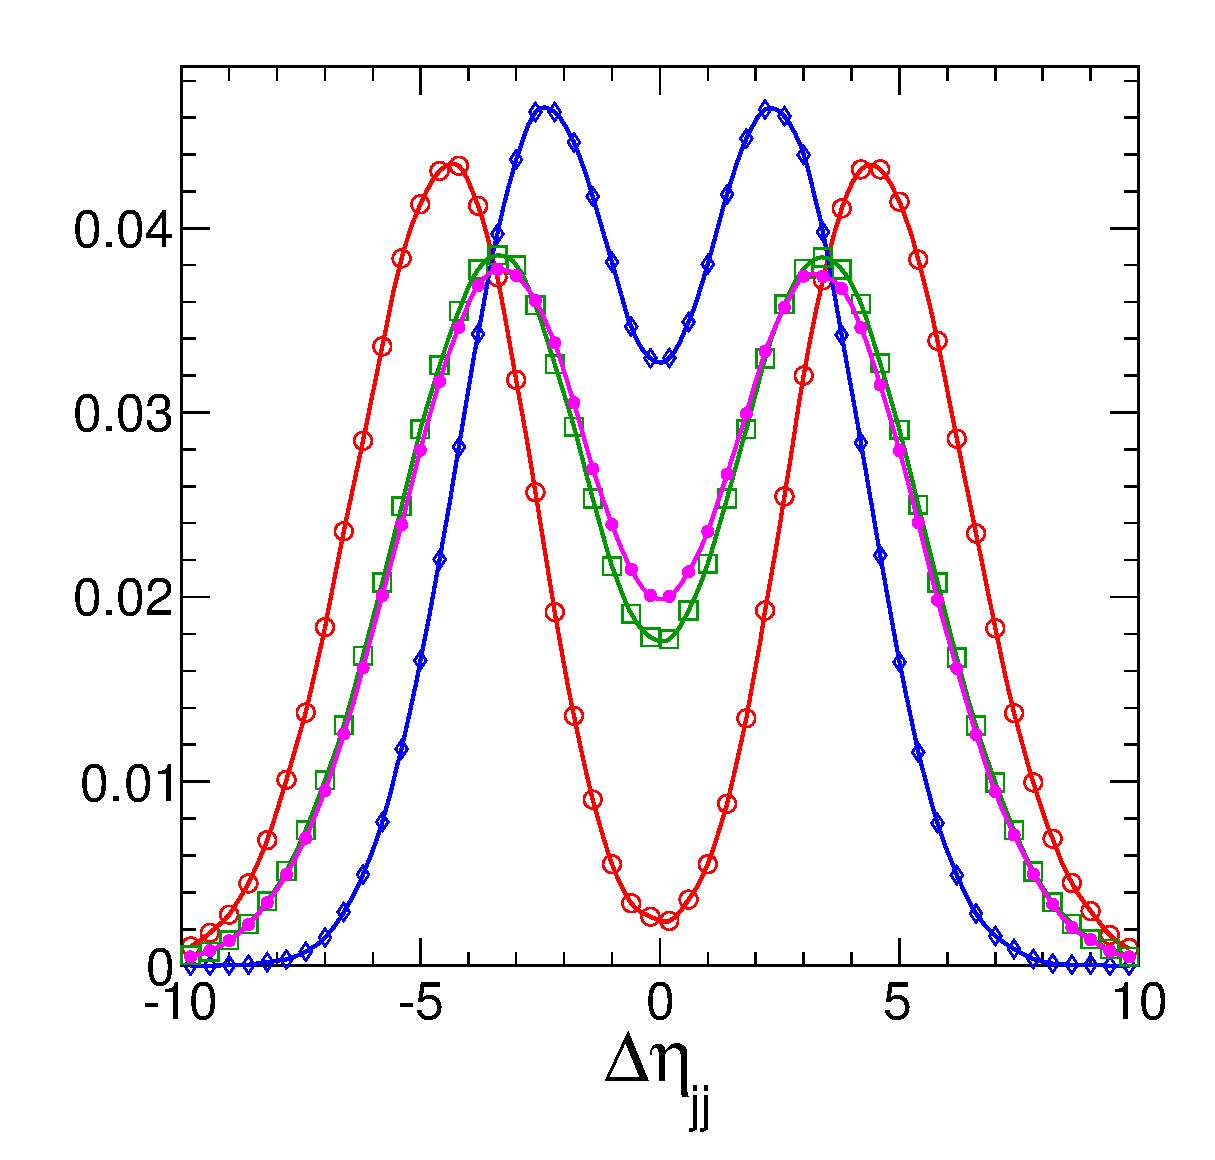
\includegraphics[width=.25\textwidth]{snowmass/14T_WBF_dEta_50}
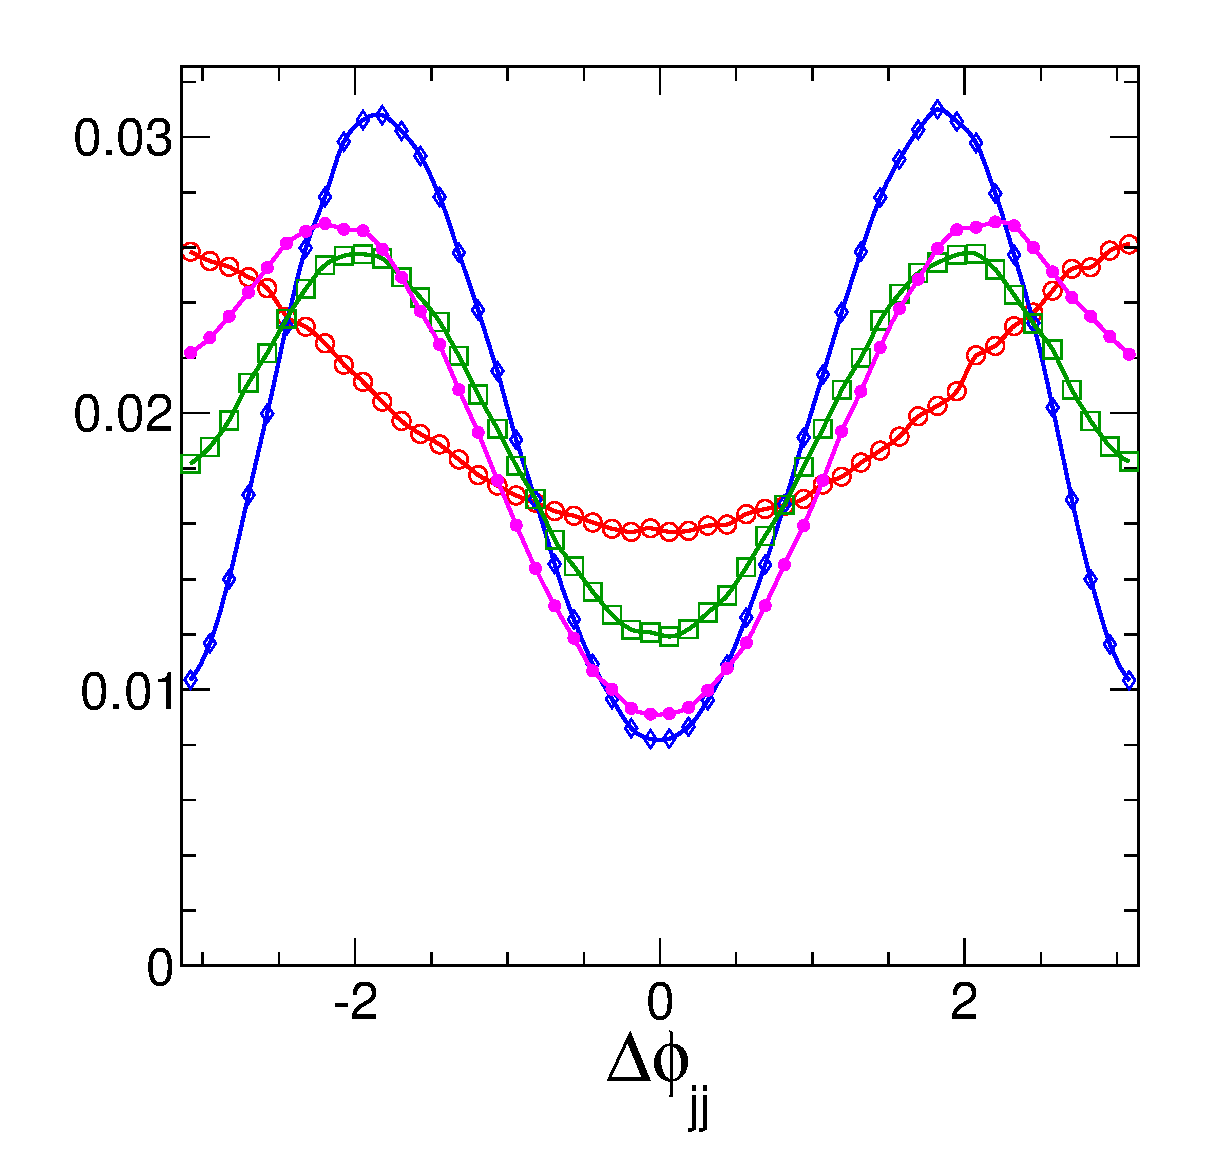
\includegraphics[width=.25\textwidth]{snowmass/14T_WBF_dPhi_50} \\
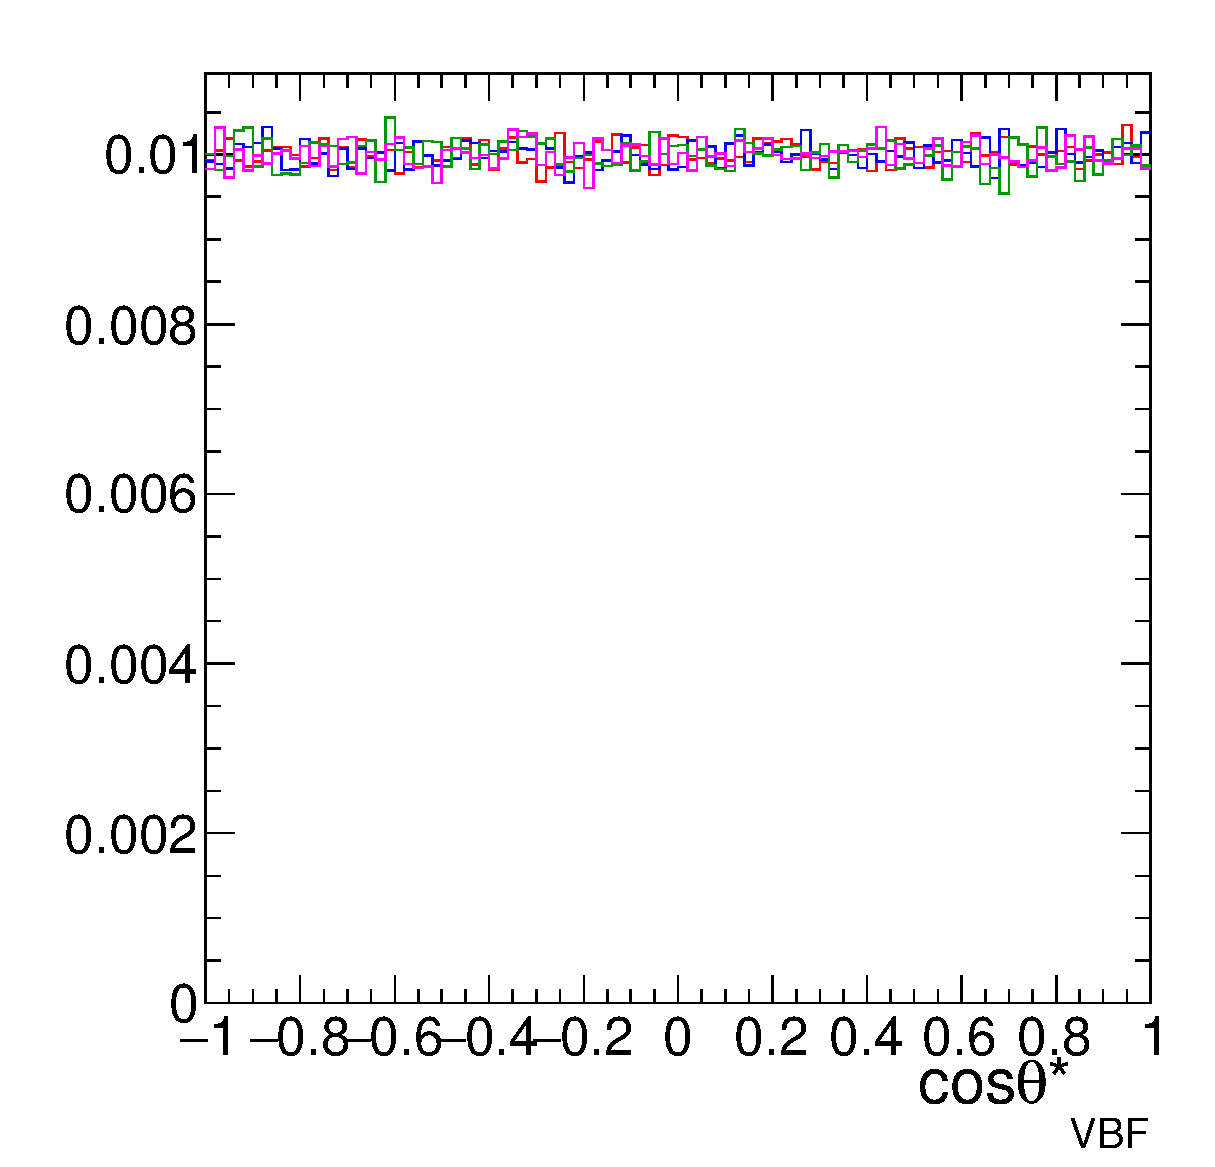
\includegraphics[width=.25\textwidth]{myplots/costhetastar}
\includegraphics[width=.25\textwidth]{myplots/costheta1}
\includegraphics[width=.25\textwidth]{myplots/Phi}
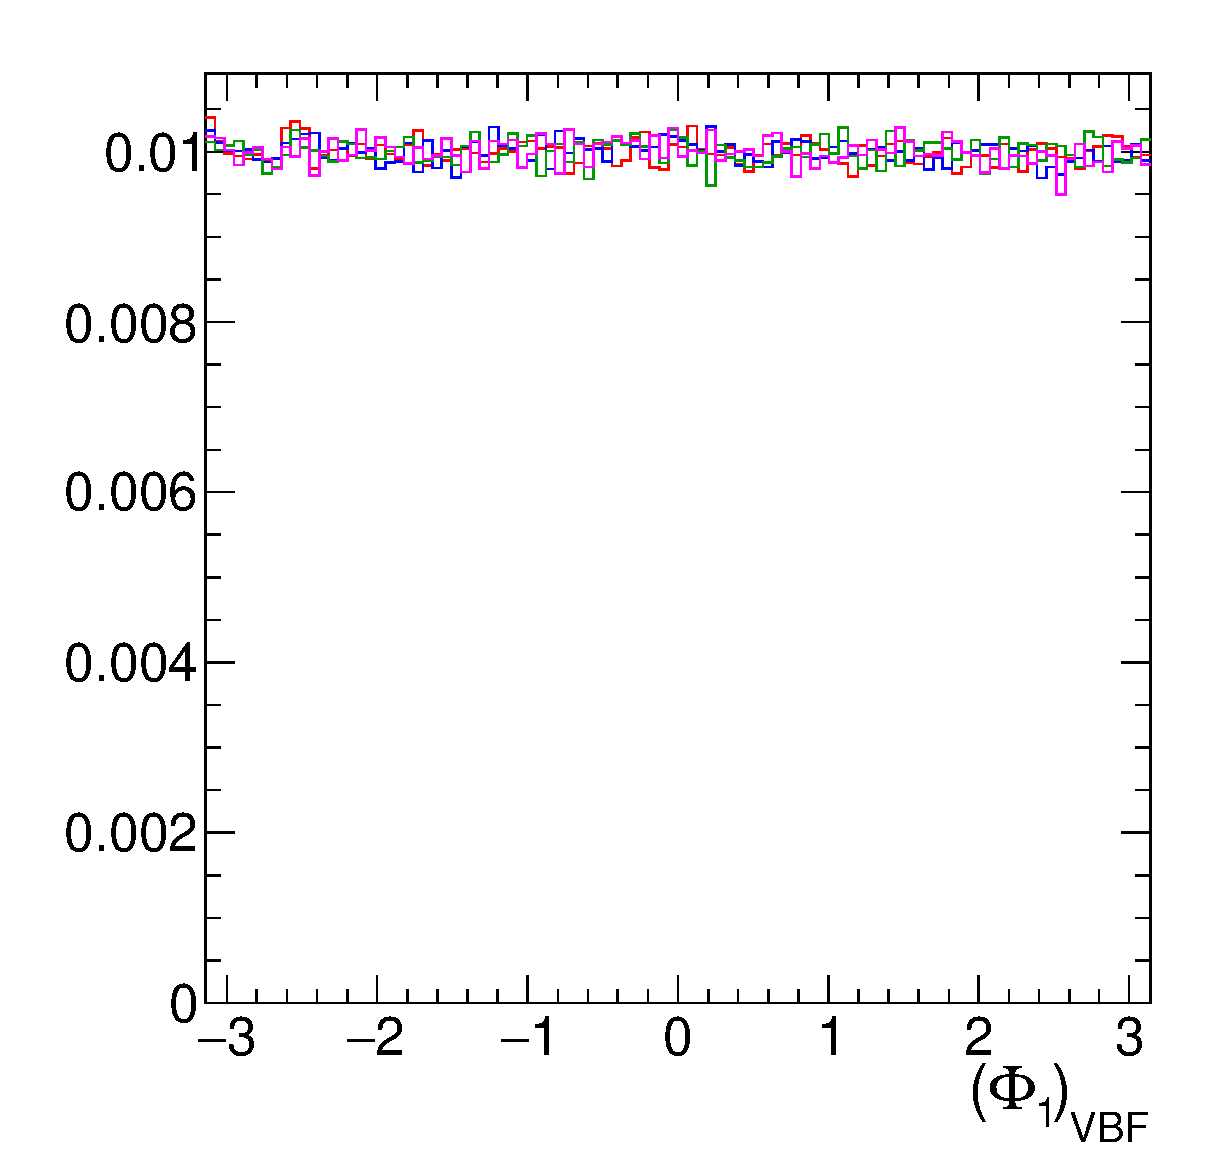
\includegraphics[width=.25\textwidth]{myplots/Phi1}
\end{frame}

\begin{frame}{Applications for discriminating CP properties}{Summary table}
\resizebox{\textwidth}{!}{
\begin{tabular}{|lcccc || cccccc || cccc |}
\hline
\hline
 \multicolumn{5}{|c||}{process description}  &  \multicolumn{6}{c||}{MC simulation parameters}  &  \multicolumn{4}{c|}{~~expected precision~~}  \\
\hline
collider & energy &  mode  &  $\sigma_2/\sigma_1$ &  $\sigma_4/\sigma_{+}$ & $|g_2/g_1|$ &  $|g_4/g_{+}|$  & ~~$f_{a2}$ &  $f_{a2}^{\rm dec}$ &  $f_{a3}$ &  $f_{a3}^{\rm dec}$
 & $\delta f_{a2}$  & $\delta f_{a2}^{\rm dec}$ & $\delta f_{a3}$  & $\delta f_{a3}^{\rm dec}$ \\
\hline\hline
any   & any       &  $H\to ZZ^*$ & 0.362 &  0.153                      & 0 & 1.20 & \multicolumn{2}{c}{0} & \multicolumn{2}{c||}{0.18}  & \multicolumn{2}{c}{--}  & \multicolumn{2}{c|}{ 0.06 }  \\
          &               &                                            &            &              &  0 & 0.67 & \multicolumn{2}{c}{0} & \multicolumn{2}{c||}{0.06} & \multicolumn{2}{c}{--}  & \multicolumn{2}{c|}{ 0.02 }  \\
          &               &                                            &            &              & 0.78 & 0& \multicolumn{2}{c}{0.18} & \multicolumn{2}{c||}{0} & \multicolumn{2}{c}{ 0.088 }  & \multicolumn{2}{c|}{ -- }  \\
          &               &                                            &            &              &  0.42 & 0 & \multicolumn{2}{c}{0.06} & \multicolumn{2}{c||}{0} & \multicolumn{2}{c}{ 0.014  }  & \multicolumn{2}{c|}{ -- } \\
\hline
any   & any       &  $H\to WW^*$ & 0.776 &  0.322                      & 0 & 1.76 & \multicolumn{2}{c}{0} & \multicolumn{2}{c||}{0.50}  & \multicolumn{2}{c}{--}  & \multicolumn{2}{c|}{ -- }  \\
          &               &                                            &            &              & 1.13 & 0& \multicolumn{2}{c}{0.50} & \multicolumn{2}{c||}{0} & \multicolumn{2}{c}{ -- }  & \multicolumn{2}{c|}{ -- }  \\
\hline
any   & any       &  $H\to\gamma\gamma, gg$ & N/A &  1.0                     & N/A & 1.0 & \multicolumn{2}{c}{0} & \multicolumn{2}{c||}{0.50}  & \multicolumn{2}{c}{--}  & \multicolumn{2}{c|}{ -- }  \\
any   & any       &  $H\to Z\gamma$ & N/A &  1.0                     & N/A  & 1.0 & \multicolumn{2}{c}{0} & \multicolumn{2}{c||}{0.50}  & \multicolumn{2}{c}{--}  & \multicolumn{2}{c|}{ -- }  \\
\hline
\hline
$pp$ & 14 TeV &  $gg\to H$                        & N/A        &  1.0       &   N/A & 1.0 &  0 & 0 & 0.50 & 0.50 & \multicolumn{2}{c}{ --  } &  0.50 & 0.50 \\
          &               &   ($H\to ZZ^*$)              &            &               &  N/A & 1.0 &  0 & 0  & 0.50 & 0.50 & \multicolumn{2}{c}{ --  } & 0.16 & 0.16 \\
\hline
$pp$ & 14 TeV &  $V^*V^*\to H$                & 14.0     &  11.3    &  0 & 0.299      &  0 & 0 & 0.50 & 0.013  & \multicolumn{2}{c}{ --  } & 0.190 &$7\!\times\!10^{-3}$ \\
          &               &   ($H\to ZZ^*$)                &            &              &   0 & 0.109 &  0 & 0  & 0.12 & 0.0018 & \multicolumn{2}{c}{ --  } & 0.036 & $6\!\times\!10^{-4}$ \\
\hline
$pp$ & 14 TeV &  $V^*V^*\to H$                            & 14.0     &  11.3       & 0 & 0.109 &  0 & 0  & 0.12 & 0.0018 & \multicolumn{2}{c}{ --  }  & 0.04 & $7\!\times\!10^{-4}$  \\
          &               &   ($H\to\gamma\gamma$)             &           &                & 0 & 0.052 &  0 & 0  & 0.030 & 0.0004 & \multicolumn{2}{c}{ --  } &  0.009 & $1.3\!\times\!10^{-4}$\\
\hline
$pp$ & 14 TeV &  $V^*\to VH$                    &  76.1     &  46.8      & 0 & 0.145   & 0 & 0  & 0.50 & 0.0032  & \multicolumn{2}{c}{ --  }  & 0.32 & $3\!\times\!10^{-3}$  \\
          &              \multicolumn{2}{c}{($V\to q\bar{q}^\prime, H\to ZZ^*$)}
                                                                            &           &                & 0  & 0.095      &  0 & 0  & 0.30 & 0.0014 & \multicolumn{2}{c}{ --  } & 0.10 & $6\!\times\!10^{-4}$  \\
\hline
%
$pp$ & 14 TeV &  $V^*\to VH$                                                                   &  76.1   &  46.8      & 0 & 0.061 & 0 & 0  & 0.15 & 0.0006 & \multicolumn{2}{c}{ --  }  & 0.09  & $4\!\times\!10^{-4}$  \\
         &            \multicolumn{2}{c}{($V\to \ell^+\ell^-, H\to b\bar{b}$)}   &           &                 &  0 & 0.049 &  0 & 0  & 0.10 &  0.0004 & \multicolumn{2}{c}{ --  } & 0.029 & $1.2\!\times\!10^{-4}$  \\
\hline\hline
$e^+e^-$ & 250 GeV & $Z^*\to ZH$ & 34.1 &  8.07 & 0  & 0.117 & 0 & 0  & 0.10 & $2\times10^{-3}$ & \multicolumn{2}{c}{ --  } & 0.032 & $7\!\times\!10^{-4}$ \\
         &               &                            &         &       &  0.057 &  0 & 0.10 & $1.2\times10^{-3}$ &  0 & 0  & 0.033 & $4\!\times\!10^{-4}$ & \multicolumn{2}{c|}{ --  }  \\
\hline
$e^+e^-$ & 350 GeV & $Z^*\to ZH$ & 84.2 &  50.6 &  0 & 0.0469 & 0 & 0  & 0.10  & $3\times10^{-4}$ & \multicolumn{2}{c}{ --  } & 0.031 &  $1.1\!\times\!10^{-4}$ \\
        &               &                            &         &       &  0.025  &  0 & 0.05 & $2\times10^{-4}$ &  0 & 0  & 0.015 & $7\!\times\!10^{-5}$   & \multicolumn{2}{c|}{ --  }   \\
\hline
$e^+e^-$ & 500 GeV & $Z^*\to ZH$ & 200.8 &  161.1 &  0 & 0.0263 & 0 & 0  & 0.10 & $1.1\times10^{-4}$ & \multicolumn{2}{c}{ --  } & 0.034 &  $4\!\times\!10^{-5}$ \\
        &               &                            &         &       &   0.024 &  0 & 0.10 & $2\times10^{-4}$  &  0 & 0  & 0.033 &  $7\!\times\!10^{-5}$ & \multicolumn{2}{c|}{ --  }   \\
\hline
$e^+e^-$ & 1 TeV     & $Z^*\to ZH$ & 916.5 &  870.8 &   0 & 0.0113 & 0 & 0 & 0.10 & $2\times10^{-5}$ & \multicolumn{2}{c}{ --  } & 0.037 &  $8\!\times\!10^{-6}$ \\
        &               &                            &                        &       &  0.014 &  0 & 0.15 & $7\times10^{-5}$  &  0 & 0  & 0.049 & $3\!\times\!10^{-5}$ & \multicolumn{2}{c|}{ --  }  \\
\hline
\hline
\end{tabular}
}
\end{frame}

\begin{frame}{$ttH$}
Study top quarks produced in association with Higgs
\includegraphics[width=.5\textwidth]{ttH/etatop}
\includegraphics[width=.5\textwidth]{ttH/pTH}
\begin{itemize}
\item Associated top production is very sensitive to the incoming partons
\begin{itemize}[label=$\Rightarrow$]
\item Include PDF in MELA weight
\[
\sim f^p_i\left(x_1\right)f^p_j\left(x_2\right)\times\left|\mathcal{M}\left(d\Pi\right)\right|^2
\]
\end{itemize}
\item Similar for VBF, VH, $H+j\left(j\right)$
\end{itemize}
\end{frame}



\begin{frame}{JHUGen in action: Generation, reweighting, discriminants}{
%twiki: https://twiki.cern.ch/twiki/bin/view/CMSPublic/Hig14018PaperTwiki
CMS analysis $H \to ZZ^*/Z\gamma^*/\gamma^*\gamma^* \to 4l$\hfill [CMS-HIG-14-018] \arxiv{1411.3441}
}
\includegraphics[width=0.25\textwidth]{HVV/d0minus}
\includegraphics[width=0.25\textwidth]{HVV/d0hplus}
\includegraphics[width=0.25\textwidth]{HVV/dlambda1}
\includegraphics[width=0.25\textwidth]{HVV/dcp}
\\
\begin{columns}
\begin{column}{0.6\textwidth}
\includegraphics[width=\textwidth]{HVV/summary_a2a3lambda1}
\end{column}
\begin{column}{0.4\textwidth}
\includegraphics[width=\textwidth]{HVV/JP_SummaryPlot}
\end{column}
\end{columns}
\end{frame}

\begin{frame}{JHUGen in action: Applications of reweighting}{CMS analysis $H \to ZZ^*/Z\gamma^*/\gamma^*\gamma^* \to 4l$\hfill [CMS-HIG-14-018] \arxiv{1411.3441}}

JHUGen generator level:
\includegraphics[width=0.25\textwidth]{HVV/SM}
\includegraphics[width=0.25\textwidth]{HVV/fa2}
\includegraphics[width=0.25\textwidth]{HVV/fa3}
\includegraphics[width=0.25\textwidth]{HVV/flambda1}
\begin{columns}
\begin{column}{0.6\textwidth}
\footnotesize
\begin{itemize}
\item Generate 24 base models
\item Create 52 target models through reweighting
\item To increase statistics:
\begin{itemize}
\item Reweight \emph{everything to everything}
\end{itemize}
\item Effectively increase sample size by $\times 24$.
\end{itemize}
\end{column}
\begin{column}{0.13\textwidth} \footnotesize
JHUGen detector level (everything reweighted to SM):
\end{column}
\begin{column}{0.27\textwidth}
\includegraphics[width=\textwidth]{HVV/reweighted}
\end{column}
\end{columns}
\end{frame}

\begin{frame}{JHUGen in action}{CMS analysis $H \to ZZ^*/Z\gamma^*/\gamma^*\gamma^* \to 4l$\hfill [CMS-HIG-14-018] \arxiv{1411.3441}}
\begin{columns}
\begin{column}{0.6\textwidth}
\includegraphics[width=.5\columnwidth]{HVV/costheta1}
\includegraphics[width=.5\columnwidth]{HVV/Phi} \\
\includegraphics[width=.5\columnwidth]{HVV/m1}
\includegraphics[width=.5\columnwidth]{HVV/m2}
\end{column}
\begin{column}{0.4\textwidth}
\begin{itemize}
\item angular and mass variables for on-shell kinematics
\item all signal distributions obtained via reweighting
\end{itemize}
\end{column}
\end{columns}
\end{frame}

\begin{frame}{JHUGen in action}{CMS analysis $H \to ZZ^*/Z\gamma^*/\gamma^*\gamma^* \to 4l$\hfill [CMS-HIG-14-018] \arxiv{1411.3441}}
\begin{columns}
\begin{column}{0.6\textwidth}
\includegraphics[width=.5\columnwidth]{HVV/d0minus}
\includegraphics[width=.5\columnwidth]{HVV/dlambda1} \\
\includegraphics[width=.5\columnwidth]{HVV/Da3gammagamma}
\includegraphics[width=.5\columnwidth]{HVV/Da2Zgamma}
\end{column}
\begin{column}{0.4\textwidth}
\begin{itemize}
\item discriminants for on-shell kinematics
\item all signal distributions obtained via reweighting
\end{itemize}
\end{column}
\end{columns}
\end{frame}

\begin{frame}{JHUGen in action}{ATLAS analysis $H \to ZZ^* \to 4l$\hfill [ATLAS-HIGG-2013-17] \arxiv{1506.05669}}
%Study of the spin and parity of the Higgs boson in diboson decays with the ATLAS detector
%https://atlas.web.cern.ch/Atlas/GROUPS/PHYSICS/PAPERS/HIGG-2013-17/
\begin{columns}
\begin{column}{0.6\textwidth}
\includegraphics[width=.5\columnwidth]{ATLASHVV/TO1}
\includegraphics[width=.5\columnwidth]{ATLASHVV/TO2} \\
\includegraphics[width=.5\columnwidth]{ATLASHVV/TO1plusTO2}
\includegraphics[width=.5\columnwidth]{ATLASHVV/TO1minusTO2}
\end{column}
\begin{column}{0.4\textwidth}
\begin{itemize}
\item Distributions of anomalous couplings were obtained by reweighting the base sample using JHUGen.
\end{itemize}
\end{column}
\end{columns}
\end{frame}

\begin{frame}{JHUGen in action}{CMS analysis $H \to WW$\hfill [CMS-HIG-14-018] \arxiv{1411.3441}}
\begin{columns}
\begin{column}{0.6\textwidth}
\includegraphics[width=.5\columnwidth]{HVV/WWmll}
\includegraphics[width=.5\columnwidth]{HVV/WWmT} \\
\includegraphics[width=.5\columnwidth]{HVV/WW1jetmll}
\includegraphics[width=.5\columnwidth]{HVV/WW1jetmT}
\end{column}
\begin{column}{0.4\textwidth}
\begin{itemize}
\item mass variables for on-shell kinematics
\item all signal distributions obtained via reweighting of all models to all models
\end{itemize}
\end{column}
\end{columns}
\end{frame}

\begin{frame}{JHUGen in action: Off-shell reweighting}{CMS Higgs off-shell analysis\hfill [CMS-HIG-14-036] \arxiv{1507.06656}}
$$\sigma^\text{on-shell}_{vv\to H\to ZZ}\sim\mu_{vvH}\therefore \sigma^\text{off-shell}_{vv\to H\to ZZ}\sim \mu_{vvH}\times\Gamma_H$$
\begin{columns}
\begin{column}{0.1\textwidth}
Gluon fusion signal only % (to be replaced with non Work in Progress from Ulascan)
\end{column}
\begin{column}{0.75\textwidth}
\includegraphics[width=0.5\columnwidth]{lifetime/signalonly}
\includegraphics[width=0.5\columnwidth]{lifetime/fig1}
\end{column}
\begin{column}{0.15\textwidth}
Gluon fusion signal + bkg. + int.
\end{column}
\end{columns}
\begin{itemize} \footnotesize
\item all signal distributions obtained via re-weighting
\item use add-on for MCFM to implement anomalous couplings and interface MELA with MCFM to include signal + background + interference
\end{itemize}
\end{frame}

\begin{frame}{JHUGen in action: Background reweighting}{H. Roskes, \emph{Validation of the Higgs boson spin-parity
analysis with $Z\to 4l$ data}\\ \url{http://meetings.aps.org/link/BAPS.2015.APR.X16.8}}
\begin{columns}
\begin{column}{0.55\textwidth}
\includegraphics[width=.5\columnwidth]{HVV/Z4lmH}
\includegraphics[width=.5\columnwidth]{HVV/Z4lcostheta1} \\
\includegraphics[width=.5\columnwidth]{HVV/Z4lm1}
\includegraphics[width=.5\columnwidth]{HVV/Z4lm2}
\end{column}
\begin{column}{0.45\textwidth}
\begin{itemize}
\item Mixture of $s$, $t$, and $u$ channels generated with POWHEG
\item MELA reweighting used $s$ and $t+u$ channels separately, along with interference
\item $gg$ background is obtained by reweighting $q\bar{q}$
\end{itemize}
\end{column}
\end{columns}
\end{frame}

\begin{frame}{JHUGen in action: Background reweighting}{H. Roskes, \emph{Validation of the Higgs boson spin-parity
analysis with $Z\to 4l$ data}\\ \url{http://meetings.aps.org/link/BAPS.2015.APR.X16.8}}
\begin{columns}
\begin{column}{0.55\textwidth}
\includegraphics[width=.5\columnwidth]{HVV/Z4lDbkgkin}
\includegraphics[width=.5\columnwidth]{HVV/Z4lfHscan} \\
\newlength{\imageheight}
\settoheight\imageheight{\includegraphics[width=.5\columnwidth]{HVV/Z4lftuscan}}
\hfuzz=24pt
\includegraphics[width=.5\columnwidth]{HVV/Z4lftuscan}
\includegraphics[height=\the\imageheight]{HVV/Z4l2dscan}
\end{column}
\begin{column}{0.45\textwidth}
\begin{itemize}
\item MELA discriminant $D^\text{bkg}_\text{kin}$ to separate $Z$ boson from alternative Higgs hypothesis.
\item Higgs hypothesis excluded at $>99\%$ CL
\end{itemize}
\end{column}
\end{columns}
\end{frame}

\begin{frame}{Summary}
\begin{itemize}
\item JHUGen is a flexible framework for studies of anomalous couplings in spin-0,1,2 resonance production and other associated production modes.
\begin{multicols}{2}
\begin{itemize}
\item VBF
\item $H+$1 or 2 QCD jets
\item $VH$
\item $t\bar{t}H$
\item More to come
\item %blank for alignment
\end{itemize}
\end{multicols}
\item JHUGenMELA provides respective matrix elements for:
\begin{itemize}
\item optimal discriminants for anomalous coupling fits
\item background suppression
\item re-weighting
\end{itemize}
\item Fruitful application in various analyses by CMS and ATLAS
\item Future developments:
\begin{itemize}
\item Application to more Higgs production mechanisms and decay channels
\end{itemize}
\end{itemize}
\end{frame}
\end{document}
